\chapter{ΕΡΩΤΗΜΑ 2}
    Χρησιμοποιούμε τις εξής αλυσίδες φεριττίνης:
    \begin{graycomment} \footnotesize
    \begin{verbatim}
>AAH13928.1 Ferritin, light polypeptide [Homo sapiens]
    MSSQIRQNYSTDVEAAVNSLVNLYLQASYTYLSLGFYFDRDDVALEGVSHFFRELAEEKREGYERLLKMQNQRGGRALFQ
    DIKKPAEDEWGKTPDAMKAAMALEKKLNQALLDLHALGSARTDPRLCDFLETHFLDEEVKLIKKMGDHLTNLHRLGGPEA
    GLGEYLFERLTLKHD
>NP_001126850.1 ferritin light chain [Pongo abelii]
    MSSQIRQNYSTDVEAAVNSLVNMYLQASYTYLSLGFYFDRDDVALEGVSHFFRELAEEKREGYERLLKMQNQRGGRALFQ
    DIKKPAEDEWGKTPDAMKAAMALEKKLNQALLDLHALGSAHTDPHLCDFLETHFLDEEVKLIKKMGDHLTNLHRLGGPEA
    GLGEYLFERLTLKHD
>XP_063672238.1 ferritin light chain-like [Pan troglodytes]
    MFWQFGGPAGLSLASTVFGRNRSGDSLPASDRPPISSPLATSGTIFSAISCFWDLPAPFLWLAPSCQPTMSSQIRQNYST
    DVEAAVNSLVNLYLQASYTYLSLGFYFDRDDVALEGVSHFFRELAEEKREGYERLLKMQNQRGGRALFQDIKKPAEDEWG
    KTPDAMKAAMALEKKLNQALLDLHALGSAHTDPHLCDFLETHFLDEEVKLIKKMGDHLTNLHRLGGPEAGLGEYLFERLT
    LKHD\end{verbatim}
    \end{graycomment}

    \section{ΣΤΟΙΧΙΣΗ ΑΚΟΛΟΥΘΙΩΝ}
        Για τη στοίχιση των ακολουθιών χρησιμοποιούμε το εργαλείο T-COFFEE \cite{TCoffee}.

        \begin{center} \noindent
            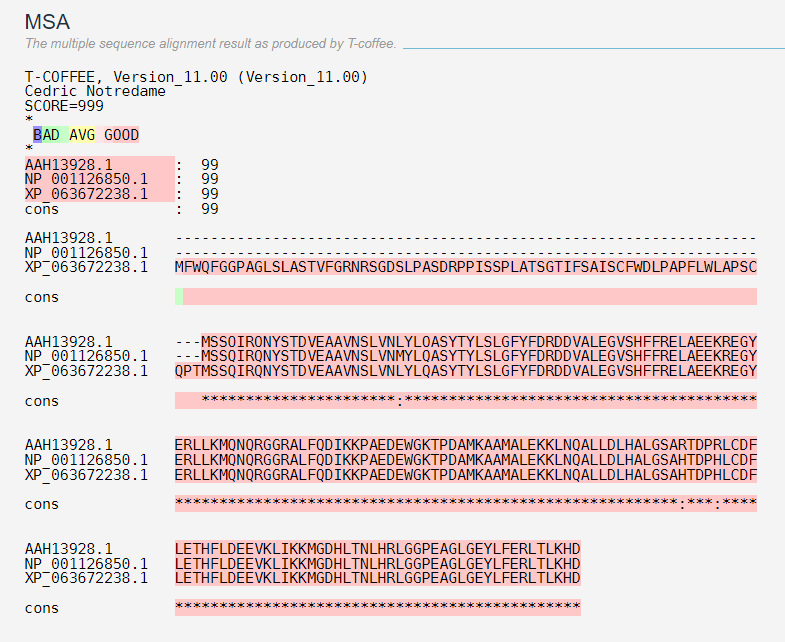
\includegraphics[scale=0.75]{img/T-Coffee}
        \end{center}

        Βλέπουμε πως υπάρχει μια πολύ καλή βαθμολογία (99), το οποίο σημαίνει πως υπάρχει μεγάλη ομοιότητα ανάμεσα στις ακολουθίες.

    \section{ΣΥΓΚΡΙΣΗ ΔΟΜΩΝ}

        \begin{center} \noindent
            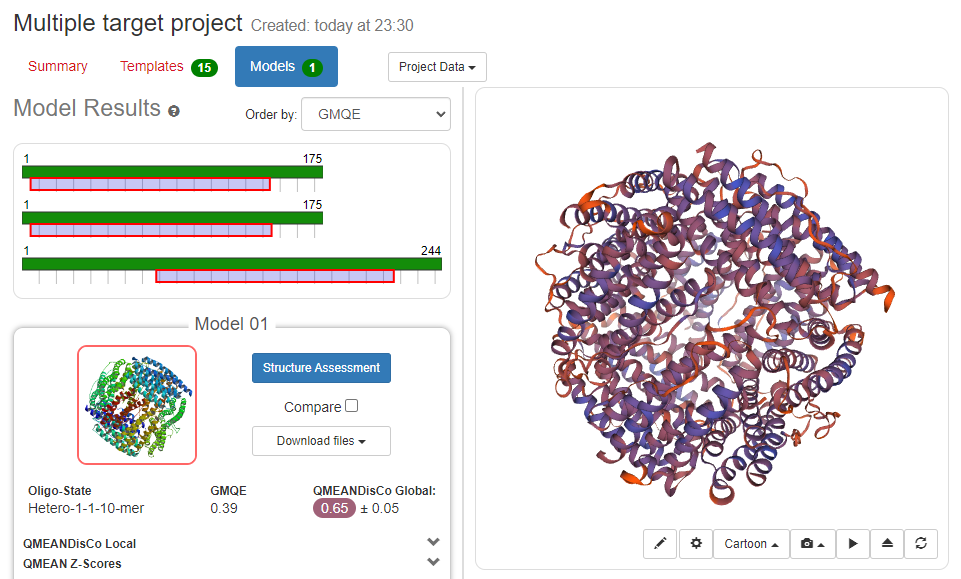
\includegraphics[scale=0.7]{img/swiss-modeller}
        \end{center}

            Αφού εξάγουμε το αρχείο \texttt{.pdb} μέσω του swiss-modeller, συγκρίνουμε τις δομές χρησιμοποιώντας το Dali.

    \begin{graycomment} \footnotesize
    \begin{verbatim}
1287:  8jb0-F 15.3  2.1  128   161   13   MOLECULE: BACTERIOFERRITIN;
1288:  8jb0-T 15.3  2.0  128   162   14   MOLECULE: BACTERIOFERRITIN;
1289:  8jb0-S 15.3  2.1  129   161   13   MOLECULE: BACTERIOFERRITIN;
1290:  2pyb-A 15.3  1.9  131   151    7   MOLECULE: NEUTROPHIL ACTIVATING PROTEIN;
1291:  6zlq-Z 15.2  2.3  136   174   75   MOLECULE: FERRITIN;
1292:  6zlq-G 15.2  2.3  136   174   75   MOLECULE: FERRITIN;
1293:  6job-B 15.2  2.4  137   172   50   MOLECULE: FERRITIN HEAVY CHAIN;
1294:  6job-A 15.2  2.4  137   172   50   MOLECULE: FERRITIN HEAVY CHAIN;
1295:  5obb-F 15.2  2.4  136   174   49   MOLECULE: FERRITIN HEAVY CHAIN;
1296:  1xz1-A 15.2  2.4  137   168   82   MOLECULE: FERRITIN LIGHT CHAIN;\end{verbatim}
    \end{graycomment}